\documentclass[12pt,a4paper]{article}

% --- Настройка языка и шрифтов для LuaLaTeX ---
\usepackage{fontspec}
\defaultfontfeatures{Ligatures=TeX,Scale=MatchLowercase}

\setmainfont{Alice-Regular}[
    Path=font/,
    Extension=.ttf,
    BoldFont = Alice-Regular,
    ItalicFont = Alice-Regular,
    BoldItalicFont = Alice-Regular,
    BoldFeatures = {FakeBold=1.6},
    ItalicFeatures = {FakeSlant=0.2},
    BoldItalicFeatures = {FakeBold=1.6,FakeSlant=0.2}
]

\newfontfamily\cyrillicfont{Alice-Regular}[
    Path=font/,
    Extension=.ttf,
    BoldFont = Alice-Regular,
    ItalicFont = Alice-Regular,
    BoldItalicFont = Alice-Regular,
    BoldFeatures = {FakeBold=1.6},
    ItalicFeatures = {FakeSlant=0.2},
    BoldItalicFeatures = {FakeBold=1.6,FakeSlant=0.2}
]

\usepackage{polyglossia}
\setmainlanguage{russian}
\setsansfont{TeX Gyre Heros}
\setmonofont{TeX Gyre Cursor}
\newfontfamily\TeXGyreTermes{TeX Gyre Termes}
\newfontfamily\TeXGyrePagella{TeX Gyre Pagella}
\newfontfamily\XCharter{XCharter}

\usepackage{graphicx}        					          % Графика
\usepackage[protrusion=false]{microtype}       	% Микротипографика
\usepackage{amsmath, amsfonts, amssymb, amsthm}	% Математика
\usepackage{braket} 							              % Braket нотация для квантовой механики
\usepackage{unicode-math} 						          % Современный пакет для математики в LuaLaTeX
\usepackage{longtable}       					          % Таблицы с разрывом страниц
\usepackage{tikz}           					          % Рисование
\usepackage[europeanresistors]{circuitikz}		  % Рисование электрических схем в европейском стиле
\usepackage{listings}							              % Для отображения кода
\usepackage{tabularx}       					          % Для таблиц во всю ширину
\usepackage{multirow}
\usepackage{array}		  						            % Для расширенных возможностей таблиц
\usepackage{float}          					          % Для точного позиционирования фигур
\usepackage{pgfplots}                           % Для построения графиков
\usepackage{caption}                            % Для настройки подписей к рисункам и таблицам
\usepackage{xfp}                                % Для вычислений в LaTeX
\pgfplotsset{compat=1.18}
\usepackage[a4paper,left=20mm,right=20mm,top=20mm,bottom=20mm]{geometry}

\usetikzlibrary{arrows.meta}

% --- Колонтитулы ---
\usepackage{fancyhdr}
\pagestyle{fancy}
\fancyhf{}

\renewcommand{\headrulewidth}{0.4pt}
\renewcommand{\footrulewidth}{0.4pt}
\renewcommand\lstlistingname{Исходный код}

\lstdefinestyle{main}{
	backgroundcolor=\color{gray!8},   
	commentstyle=\color{green!50!black},
	keywordstyle=\color{blue!80!black},
	numberstyle=\small\color{darkgray},
	stringstyle=\rmfamily\color{orange!90!black},
	basicstyle=\ttfamily\small,
	breakatwhitespace=false,         
	breaklines=true,                   
	keepspaces=true,                 
	numbers=left,                    
	numbersep=8pt,                  
	showspaces=false,                
	showstringspaces=false,
	showtabs=false,                  
	tabsize=4
}	

\lstset{style=main}

\newcolumntype{C}{>{\centering\arraybackslash}X}
\newcolumntype{J}{>{\arraybackslash}X}
\renewcommand{\arraystretch}{1.25}

% =========================================================
%         СЛУЖЕБНЫЕ КОМАНДЫ ДЛЯ ВЫЧИСЛЕНИЙ
% =========================================================
\newcommand{\CalcTwo}  [1]{\fpeval{round((#1),2)}}
\newcommand{\CalcThree}[1]{\fpeval{round((#1),3)}}
\newcommand{\CalcFour} [1]{\fpeval{round((#1),4)}}
\newcommand{\CalcFive} [1]{\fpeval{round((#1),5)}}

\def\VariantN{4}
\def\LabNumber{2}
\def\Discipline{Метрология}
\def\LabTitle{Измерительные сигналы}

\def\Vpp{1.4}
\def\VDC{0.4}
\def\fSignal{4000}
\def\KCHone{0.2}
\def\KT{0.1}
\def\Vrange{2}
\def\S{2.5}
\def\RV{1000000}
\def\RVText{$\fpeval{\RV * 10^{-6}}$ МОм}

\def\ProblemTwoGarmonicVppOne {1.45630}
\def\ProblemTwoGarmonicVRMSOne{0.63392}
\def\ProblemTwoGarmonicVRMSTwo{0.49554}
\def\ProblemTwoGarmonicVAvg{0.40094}

\def\ProblemTwoTriangularVppOne {1.42190}
\def\ProblemTwoTriangularVRMSOne{0.56568}
\def\ProblemTwoTriangularVRMSTwo{0.40467}
\def\ProblemTwoTriangularVAvg{0.40083}

\def\ProblemTwoMeanderVppOne {1.59420}
\def\ProblemTwoMeanderVRMSOne{0.80456}
\def\ProblemTwoMeanderVRMSTwo{0.69984}
\def\ProblemTwoMeanderVAvg{0.40090}

\def\ProblemTwoRectangularVppOne {1.60280}
\def\ProblemTwoRectangularVRMSOne{0.60820}
\def\ProblemTwoRectangularVRMSTwo{0.60529}
\def\ProblemTwoRectangularVAvg{0.04955}

\def\ProblemThreeResistance{456.46}
\def\ProblemThreeHighVppOne {1.46490}
\def\ProblemThreeHighVRMSOne{0.63444}
\def\ProblemThreeHighVRMSTwo{0.49473}
\def\ProblemThreeLowVppOne {1.49080}
\def\ProblemThreeLowVRMSOne{0.68144}
\def\ProblemThreeLowVRMSTwo{0.50620}

\def\ProblemFourCapacitance{0.00000000147}
\def\ProblemFourLowVppOne {1.49940}
\def\ProblemFourLowVRMSOne{0.65062}
\def\ProblemFourLowVRMSTwo{0.50702}
\def\ProblemFourHighVppOne {1.45630}
\def\ProblemFourHighVRMSOne{0.63614}
\def\ProblemFourHighVRMSTwo{0.49543}

\def\KTrust{1.1}
\def\RGenerator{50}
\def\DMMACa{0.002}
\def\DMMACb{0.0005}
\def\DMMOhma{0.0002}
\def\DMMOhmAddTwoK{0.06}
\def\DMMTwoWireAdd{0.2}
\def\CapRelErr{0.0136}

\edef\ThetaACGarm{\fpeval{\KTrust*sqrt((\DMMACa*\ProblemTwoGarmonicVRMSTwo+\DMMACb*\Vrange)^2+(0.0005*\Vrange)^2)}}
\edef\ThetaACTriangular{\fpeval{\KTrust*sqrt((\DMMACa*\ProblemTwoTriangularVRMSTwo+\DMMACb*\Vrange)^2+(0.0005*\Vrange)^2)}}
\edef\ThetaACMeander{\fpeval{abs(\DMMACa*\ProblemTwoMeanderVRMSTwo+\DMMACb*\Vrange)}}
\edef\ThetaACRectangular{\fpeval{\KTrust*sqrt((\DMMACa*\ProblemTwoRectangularVRMSTwo+\DMMACb*\Vrange)^2+(0.0005*\Vrange)^2)}}

\edef\UGarmTotal{\fpeval{sqrt(\ProblemTwoGarmonicVRMSTwo^2+\ProblemTwoGarmonicVAvg^2)}}
\edef\UTriangularTotal{\fpeval{sqrt(\ProblemTwoTriangularVRMSTwo^2+\ProblemTwoTriangularVAvg^2)}}
\edef\UMeanderTotal{\fpeval{sqrt(\ProblemTwoMeanderVRMSTwo^2+\ProblemTwoMeanderVAvg^2)}}
\edef\URectangularTotal{\fpeval{sqrt(\ProblemTwoRectangularVRMSTwo^2+\ProblemTwoRectangularVAvg^2)}}

\edef\ThetaRBase{\fpeval{\DMMOhma*\ProblemThreeResistance+\DMMOhmAddTwoK}}
\edef\ThetaR{\fpeval{\KTrust*sqrt(\ThetaRBase^2+\DMMTwoWireAdd^2)}}
\edef\GeneratorDropRel{\fpeval{\RGenerator/(\RGenerator+\ProblemThreeResistance)}}
\edef\GeneratorLoadVppCalc{\fpeval{\ProblemThreeHighVppOne*\ProblemThreeResistance/(\RGenerator+\ProblemThreeResistance)}}
\edef\GeneratorMeasuredDiffVpp{\fpeval{abs(\ProblemThreeLowVppOne-\ProblemThreeHighVppOne)}}
\edef\GeneratorMeasuredDiffRel{\fpeval{\GeneratorMeasuredDiffVpp/\ProblemThreeHighVppOne}}

\edef\FCutCalc{\fpeval{1/(2*pi*\ProblemThreeResistance*\ProblemFourCapacitance)}}
\edef\FCutExp{\fpeval{\FCutCalc*1.008}}
\edef\FLow{\fpeval{0.01*\FCutCalc}}
\edef\FHigh{\fpeval{100*\FCutCalc}}
\edef\FCutCalcKHz{\fpeval{\FCutCalc*10^(-3)}}
\edef\FCutExpKHz{\fpeval{\FCutExp*10^(-3)}}
\edef\FLowKHz{\fpeval{\FLow*10^(-3)}}
\edef\FHighKHz{\fpeval{\FHigh*10^(-3)}}
\edef\FHighMHz{\fpeval{\FHigh*10^(-6)}}
\edef\ThetaFRel{\fpeval{sqrt((\ThetaR/\ProblemThreeResistance)^2+\CapRelErr^2)}}
\edef\ThetaF{\fpeval{\ThetaFRel*\FCutCalc}}
\edef\ThetaFKHz{\fpeval{\ThetaF*10^(-3)}}

\edef\FTableSixOne{\fpeval{\FCutExpKHz}}
\edef\FTableSixTwo{\fpeval{\FCutExpKHz - (\FCutExpKHz-\FLowKHz)/10}}
\edef\FTableSixThree{\fpeval{\FCutExpKHz - 2*(\FCutExpKHz-\FLowKHz)/10}}
\edef\FTableSixFour{\fpeval{\FCutExpKHz - 3*(\FCutExpKHz-\FLowKHz)/10}}
\edef\FTableSixFive{\fpeval{\FCutExpKHz - 4*(\FCutExpKHz-\FLowKHz)/10}}
\edef\FTableSixSix{\fpeval{\FCutExpKHz - 5*(\FCutExpKHz-\FLowKHz)/10}}
\edef\FTableSixSeven{\fpeval{\FCutExpKHz - 6*(\FCutExpKHz-\FLowKHz)/10}}
\edef\FTableSixEight{\fpeval{\FCutExpKHz - 7*(\FCutExpKHz-\FLowKHz)/10}}
\edef\FTableSixNine{\fpeval{\FCutExpKHz - 8*(\FCutExpKHz-\FLowKHz)/10}}
\edef\FTableSixTen{\fpeval{\FCutExpKHz - 9*(\FCutExpKHz-\FLowKHz)/10}}
\edef\FTableSixEleven{\fpeval{\FLowKHz}}

\def\ProblemFourCutVoutOne{1.0260}
\def\ProblemFourCutVinOne{1.4557}
\def\ProblemFourCutVRMSTwoOne{0.34923}
\def\ProblemFourCutVoutTwo{1.0770}
\def\ProblemFourCutVinTwo{1.4576}
\def\ProblemFourCutVRMSTwoTwo{0.36630}
\def\ProblemFourCutVoutThree{1.1326}
\def\ProblemFourCutVinThree{1.4550}
\def\ProblemFourCutVRMSTwoThree{0.38563}
\def\ProblemFourCutVoutFour{1.1867}
\def\ProblemFourCutVinFour{1.4572}
\def\ProblemFourCutVRMSTwoFour{0.40357}
\def\ProblemFourCutVoutFive{1.2423}
\def\ProblemFourCutVinFive{1.4548}
\def\ProblemFourCutVRMSTwoFive{0.42275}
\def\ProblemFourCutVoutSix{1.2936}
\def\ProblemFourCutVinSix{1.4569}
\def\ProblemFourCutVRMSTwoSix{0.43982}
\def\ProblemFourCutVoutSeven{1.3462}
\def\ProblemFourCutVinSeven{1.4556}
\def\ProblemFourCutVRMSTwoSeven{0.45824}
\def\ProblemFourCutVoutEight{1.3887}
\def\ProblemFourCutVinEight{1.4578}
\def\ProblemFourCutVRMSTwoEight{0.47230}
\def\ProblemFourCutVoutNine{1.4246}
\def\ProblemFourCutVinNine{1.4553}
\def\ProblemFourCutVRMSTwoNine{0.48483}
\def\ProblemFourCutVoutTen{1.4456}
\def\ProblemFourCutVinTen{1.4567}
\def\ProblemFourCutVRMSTwoTen{0.49156}
\def\ProblemFourCutVoutEleven{1.4576}
\def\ProblemFourCutVinEleven{1.4574}
\def\ProblemFourCutVRMSTwoEleven{0.49597}

\def\ProblemFiveLPFVoutOne{1.4446}
\def\ProblemFiveLPFVinOne{1.4569}
\def\ProblemFiveLPFVoutTwo{1.0618}
\def\ProblemFiveLPFVinTwo{1.4562}
\def\ProblemFiveLPFVoutThree{0.7419}
\def\ProblemFiveLPFVinThree{1.4576}

\def\ProblemSixHPFVoutOne{1.4432}
\def\ProblemSixHPFVinOne{1.4568}
\def\ProblemSixHPFVoutTwo{1.0464}
\def\ProblemSixHPFVinTwo{1.4559}
\def\ProblemSixHPFVoutThree{0.7387}
\def\ProblemSixHPFVinThree{1.4565}

\title{МИНОБРНАУКИ РОССИИ\\[0.7em]
федеральное государственное автономное образовательное учреждение\\
высшего образования\\
«Национальный исследовательский университет\\
«Московский институт электронной техники»\\[2em]}
\author{}
\date{}

\begin{document}
\maketitle
\thispagestyle{fancy}

\begin{center}
\Large Отчёт по Лабораторной работе $\LabNumber$\\
по дисциплине «\Discipline»\\
«\LabTitle»
\end{center}

\begin{center}
\Large Вариант \VariantN
\end{center}

\vspace{12em}

\begin{flushright}
Выполнили студенты группы ЭН-$25$\\
Андреев И. А.\\
Анисимов А. С.\\
Проверил преподаватель\\
Туринцев К. А.
\end{flushright}

\cfoot{Москва 2026}

\pagebreak
\fancyhead[L]{Оглавление}
\fancyhead[R]{\LabTitle}
\fancyfoot[C]{\thepage}
\tableofcontents
\pagebreak

\fancyhead[L]{Теория}
\fancyhead[R]{\LabTitle}

\begin{center}
\Large\textbf{Лабораторная работа $\LabNumber$}
\end{center}

\begin{center}
\LARGE\textbf{\LabTitle}
\end{center}

\large\textbf{\textit{Цель работы}:} постановка экспериментов по оценке параметров измерительных сигналов с использованием функционального генератора, цифрового мультиметра и цифрового осциллографа с последующей оценкой погрешностей данных измерений.

\large\textbf{\textit{Необходимое оборудование}:} цифровой мультиметр (\textbf{Rigol DM$3058$}), генератор сигналов (\textbf{Rigol DG$1022$Z}), цифровой осциллограф (\textbf{Rigol MSO$5102$}), макетная плата, кабели, перемычки, щупы и RC-цепь.


\section{Теоретические сведения}

\subsection{Измерительные сигналы}

Измерительный сигнал --- физический процесс, содержащий информацию об объекте измерения. В электрорадиоизмерениях чаще всего рассматриваются электрические измерительные сигналы, представляющие собой изменение напряжения во времени. В данной работе используются детерминированные периодические сигналы стандартной формы: гармонический сигнал, треугольный сигнал, меандр и прямоугольный сигнал со скважностью $q = 4$.

Напряжение измерительного сигнала
\begin{equation*}
u = u(t)
\end{equation*}

Периодический сигнал повторяется через промежуток времени $T$, связанный с частотой $f$
\begin{equation*}
T = \frac{1}{f}
\end{equation*}

К основным параметрам периодического сигнала относятся амплитуда, частота, период, фаза, среднее значение, полный размах и среднеквадратическое значение. Осциллограф позволяет наблюдать форму сигнала и измерять его размах, а мультиметр в режиме ACV измеряет действующее значение переменной составляющей сигнала.

\subsection{Масштабные параметры сигнала}

Полный размах напряжения $V_{pp}$ характеризует разность между максимальным и минимальным мгновенными значениями сигнала
\begin{equation*}
V_{pp}=U_{\max}-U_{\min}
\end{equation*}

Среднее значение напряжения $U_{\text{ср}}$ показывает постоянную составляющую сигнала за период усреднения
\begin{equation*}
U_{\text{ср}}=\frac{1}{T}\int\limits_0^T u(t)\,dt
\end{equation*}

Среднеквадратическое значение напряжения $U_{RMS}$ соответствует действующему значению сигнала, эквивалентному постоянному напряжению по мощности на активной нагрузке
\begin{equation*}
U_{RMS}=\sqrt{\frac{1}{T}\int\limits_0^T u^2(t)\,dt}
\end{equation*}

Полное среднеквадратическое значение при наличии постоянной и переменной составляющих
\begin{equation}
U_{\Sigma}=\sqrt{U_{RMS,AC}^2+U_{DC}^2}
\label{eq:utotal}
\end{equation}

Для гармонического сигнала без смещения
\begin{equation*}
U_{RMS,\sin}=\frac{V_{pp}}{2\sqrt2}
\end{equation*}

Для треугольного сигнала без смещения
\begin{equation*}
U_{RMS,\triangle}=\frac{V_{pp}}{2\sqrt3}
\end{equation*}

Для меандра без смещения
\begin{equation*}
U_{RMS,\square}=\frac{V_{pp}}{2}
\end{equation*}

\subsection{Генератор сигналов и нагрузка}

Генератор сигналов формирует электрические сигналы с заданными параметрами: формой, частотой, полным размахом и постоянным смещением. Внутреннее выходное сопротивление генератора в данной работе принимается равным $R_{\text{вых}}=50$ Ом. При подключении внешней нагрузки генератор и нагрузка образуют делитель напряжения, поэтому несоответствие фактической нагрузки настройке генератора приводит к методической погрешности.

Методическая погрешность генератора при подключении низкоомной нагрузки
\begin{equation}
\gamma_{\text{мет}}=\frac{R_{\text{вых}}}{R_{\text{вых}}+R_{\text{н}}}\cdot100\%
\label{eq:gen-method}
\end{equation}

Напряжение на нагрузке без компенсации настройки выхода генератора
\begin{equation}
V_{pp,\text{н}}=V_{pp,0}\frac{R_{\text{н}}}{R_{\text{вых}}+R_{\text{н}}}
\label{eq:gen-load}
\end{equation}

\subsection{Цифровой мультиметр и осциллограф}

Цифровой мультиметр используется для измерения действующего значения переменного напряжения и среднего значения напряжения по постоянной составляющей. В режиме измерения переменного напряжения мультиметр обладает входным сопротивлением $R_V=1$ МОм и конечной полосой пропускания, поэтому на высоких частотах и для несинусоидальных сигналов необходимо учитывать дополнительные составляющие погрешности.

Цифровой осциллограф используется как средство контроля формы сигнала, полного размаха, частоты и действующего значения. В данной работе показания осциллографа принимаются как опорные при сравнении с показаниями мультиметра, так как осциллограф одновременно отображает форму сигнала и позволяет убедиться в корректности настройки генератора.

\subsection{Погрешности измерения параметров сигналов}

Абсолютная погрешность измерения $\Delta x$
\begin{equation*}
\Delta x=x_{\text{изм}}-x_{\text{оп}}
\end{equation*}

Относительная погрешность измерения $\delta$
\begin{equation*}
\delta=\frac{|\Delta x|}{x_{\text{изм}}}\cdot100\%
\end{equation*}

Суммарная инструментальная погрешность при доверительной вероятности $P=95\%$
\begin{equation*}
\Theta=\pm1.1\sqrt{\theta_1^2+\theta_2^2+\ldots+\theta_n^2}
\end{equation*}

Основная погрешность мультиметра в режиме измерения переменного напряжения
\begin{equation*}
\theta_{AC}=\pm\left(0.002U_{RMS2}+0.0005U_{\text{предел}}\right)
\end{equation*}

Суммарная погрешность мультиметра с учетом погрешности, связанной с крест-фактором сигнала
\begin{equation}
\Theta_{AC}=\pm1.1\sqrt{\theta_{AC}^2+\theta_{CF}^2}
\label{eq:dmm-ac-full}
\end{equation}

\subsection{RC-цепь как измерительный преобразователь}

RC-цепь используется как частотно-зависимый измерительный преобразователь. В зависимости от точки съема выходного напряжения она работает как фильтр низких частот или фильтр высоких частот. В режиме ФНЧ выходное напряжение снимается с конденсатора, поэтому низкочастотные составляющие проходят почти без ослабления, а высокочастотные подавляются. В режиме ФВЧ выходное напряжение снимается с резистора, поэтому высокочастотные составляющие проходят почти без ослабления, а низкочастотные подавляются.

Импеданс последовательной RC-цепи
\begin{equation*}
Z_{RC}=R+\frac{1}{j\omega C}
\end{equation*}

Частота среза RC-цепи
\begin{equation}
f_{\text{ср}}=\frac{1}{2\pi RC}
\label{eq:fcut}
\end{equation}

Коэффициент передачи ФНЧ
\begin{equation*}
K_{\text{ФНЧ}}(f)=\frac{1}{\sqrt{1+\left(\frac{f}{f_{\text{ср}}}\right)^2}}
\end{equation*}

Коэффициент передачи ФВЧ
\begin{equation*}
K_{\text{ФВЧ}}(f)=\frac{\frac{f}{f_{\text{ср}}}}{\sqrt{1+\left(\frac{f}{f_{\text{ср}}}\right)^2}}
\end{equation*}

На частоте среза выходной размах одиночной гармонической составляющей уменьшается в $\sqrt2$ раза
\begin{equation}
\frac{V_{\text{вх}}}{V_{\text{вых}}}=\sqrt2
\label{eq:sqrt2}
\end{equation}

Погрешность косвенного определения частоты среза по результатам измерения сопротивления и емкости
\begin{equation}
\frac{\Theta_f}{f_{\text{ср}}}=\sqrt{\left(\frac{\Theta_R}{R}\right)^2+\left(\frac{\Theta_C}{C}\right)^2}
\label{eq:fcut-error}
\end{equation}

\pagebreak

\begin{center}
\LARGE{\textbf{Выполнение лабораторной работы и расчетно-графическая часть}}
\end{center}

\fancyhead[L]{Задание $2$}
\section{Измерение напряжения переменного тока на выходе генератора сигналов}

\subsection{Схема и протокол измерительного эксперимента}

Схема измерительного эксперимента представлена на рис.~\ref{fig:signal-measure}. Осциллограф контролирует форму, полный размах и действующее значение сигнала; мультиметр измеряет переменную и постоянную составляющие напряжения.

\begin{figure}[H]
\centering
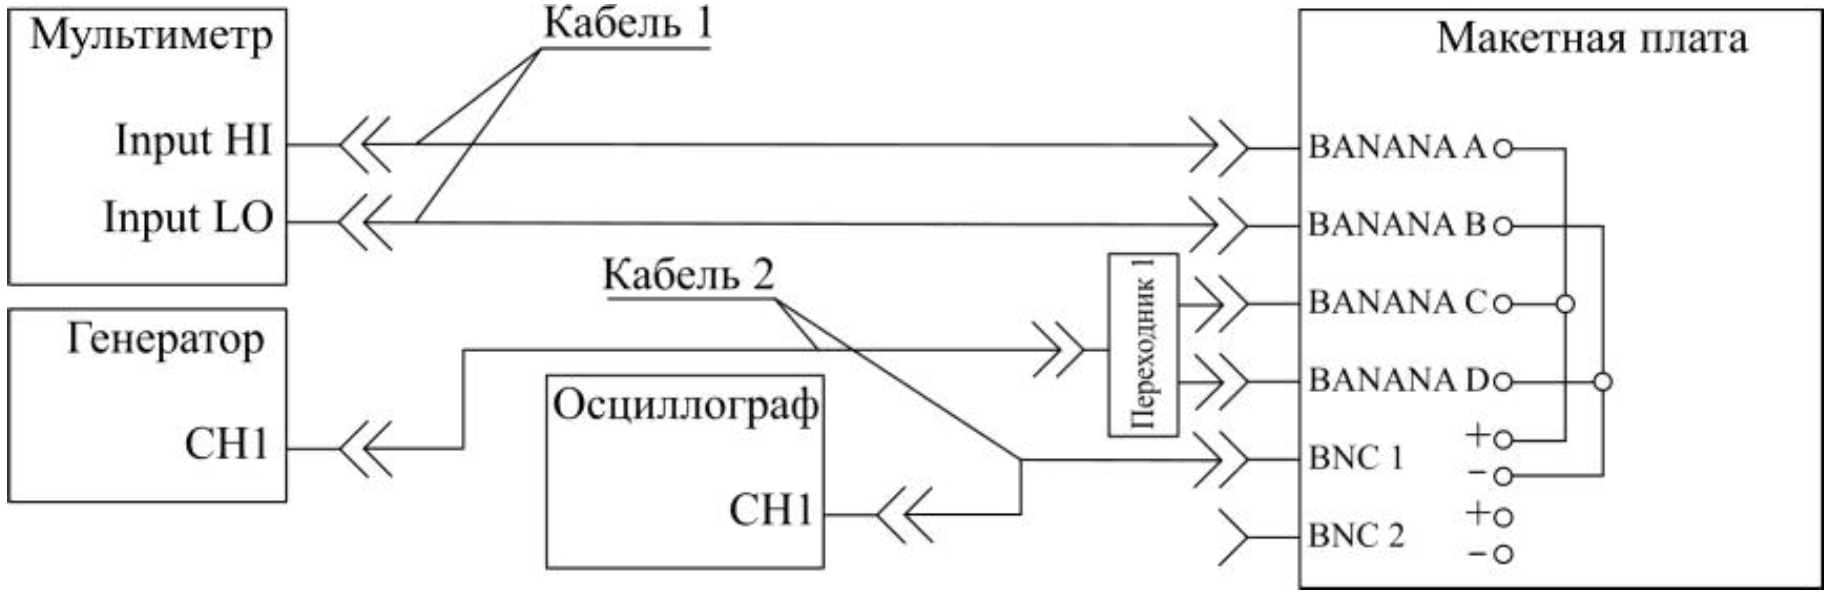
\includegraphics[width=0.92\textwidth]{01scheme.png}
\caption{Схема измерения напряжения переменного тока на выходе генератора сигналов}
\label{fig:signal-measure}
\end{figure}

\begin{table}[H]
\caption{Протокол измерения выходного сигнала генератора}
\label{tab:a21}
\begin{tabularx}{\textwidth}{|J|C|C|C|C|}
\hline
\multicolumn{2}{|p{4cm}|}{Генератор сигналов} & $V_{pp}$: $\Vpp$ В & $V_{DC}$: $\VDC$ В & $f_\text{сигн}$: $\fpeval{\fSignal * 10^{-3}}$ кГц \\
\hline
\multicolumn{2}{|p{4cm}|}{Осциллограф} & $K_{CH1}$: $\KCHone$ В/дел & $K_T$: $\KT$ мс/дел & \\
\hline
\multicolumn{2}{|p{4cm}|}{Мультиметр} & Диапазон: $\Vrange$ В & $\nu$: $\S$ изм/с & $R_V$: \RVText \\
\hline
\multirow{2}{*}{Форма сигнала} & \multicolumn{2}{c|}{Показания осциллографа} & \multicolumn{2}{c|}{Показания мультиметра} \\
\cline{2-5}
& $V_{pp1}$, В & $V_{RMS1}$, В & $V_{RMS2}$, В & $V_{\text{ср}}$, В \\
\hline
Гармонический & $\ProblemTwoGarmonicVppOne$ & $\ProblemTwoGarmonicVRMSOne$ & $\ProblemTwoGarmonicVRMSTwo$ & $\ProblemTwoGarmonicVAvg$ \\
\hline
Треугольный & $\ProblemTwoTriangularVppOne$ & $\ProblemTwoTriangularVRMSOne$ & $\ProblemTwoTriangularVRMSTwo$ & $\ProblemTwoTriangularVAvg$ \\
\hline
Меандр & $\ProblemTwoMeanderVppOne$ & $\ProblemTwoMeanderVRMSOne$ & $\ProblemTwoMeanderVRMSTwo$ & $\ProblemTwoMeanderVAvg$ \\
\hline
\small Прямоугольный, скважность $q = 4$ & \raisebox{-0.5em}{$\ProblemTwoRectangularVppOne$} & \raisebox{-0.5em}{$\ProblemTwoRectangularVRMSOne$} & \raisebox{-0.5em}{$\ProblemTwoRectangularVRMSTwo$} & \raisebox{-0.5em}{$\ProblemTwoRectangularVAvg$} \\
\hline
\end{tabularx}
\end{table}

\subsection{Оценка погрешностей мультиметра}

Погрешность измерения гармонического сигнала по \eqref{eq:dmm-ac-full}
\begin{equation*}
\Theta_{AC,\sin}=\pm1.1\sqrt{\theta_{AC,\sin}^2+\theta_{CF,\sin}^2}
\end{equation*}
\begin{equation*}
\Theta_{AC,\sin}=\pm1.1\sqrt{\left(0.002\cdot\ProblemTwoGarmonicVRMSTwo+0.0005\cdot\Vrange\right)^2+\left(0.0005\cdot\Vrange\right)^2}
\end{equation*}
\begin{equation*}
\Theta_{AC,\sin}\approx\pm\CalcFive{\ThetaACGarm}\ \text{В}
\end{equation*}

Погрешность измерения треугольного сигнала
\begin{equation*}
\Theta_{AC,\triangle}=\pm1.1\sqrt{\theta_{AC,\triangle}^2+\theta_{CF,\triangle}^2}
\end{equation*}
\begin{equation*}
\Theta_{AC,\triangle}=\pm1.1\sqrt{\left(0.002\cdot\ProblemTwoTriangularVRMSTwo+0.0005\cdot\Vrange\right)^2+\left(0.0005\cdot\Vrange\right)^2}
\end{equation*}
\begin{equation*}
\Theta_{AC,\triangle}\approx\pm\CalcFive{\ThetaACTriangular}\ \text{В}
\end{equation*}

Погрешность измерения меандра
\begin{equation*}
\Theta_{AC,\square}=\pm\left|0.002V_{RMS2}+0.0005U_{\text{предел}}\right|
\end{equation*}
\begin{equation*}
\Theta_{AC,\square}=\pm\left|0.002\cdot\ProblemTwoMeanderVRMSTwo+0.0005\cdot\Vrange\right|
\end{equation*}
\begin{equation*}
\Theta_{AC,\square}\approx\pm\CalcFive{\ThetaACMeander}\ \text{В}
\end{equation*}

Погрешность измерения прямоугольного сигнала со скважностью $q=4$
\begin{equation*}
\Theta_{AC,q=4}=\pm1.1\sqrt{\theta_{AC,q=4}^2+\theta_{CF,q=4}^2}
\end{equation*}
\begin{equation*}
\Theta_{AC,q=4}=\pm1.1\sqrt{\left(0.002\cdot\ProblemTwoRectangularVRMSTwo+0.0005\cdot\Vrange\right)^2+\left(0.0005\cdot\Vrange\right)^2}
\end{equation*}
\begin{equation*}
\Theta_{AC,q=4}\approx\pm\CalcFive{\ThetaACRectangular}\ \text{В}
\end{equation*}

Полное действующее значение гармонического сигнала по \eqref{eq:utotal}
\begin{equation*}
U_{\Sigma,\sin}=\sqrt{V_{RMS2}^2+V_{\text{ср}}^2}
\end{equation*}
\begin{equation*}
U_{\Sigma,\sin}=\sqrt{\ProblemTwoGarmonicVRMSTwo^2+\ProblemTwoGarmonicVAvg^2}
\end{equation*}
\begin{equation*}
U_{\Sigma,\sin}\approx\CalcFive{\UGarmTotal}\ \text{В}
\end{equation*}

Полное действующее значение треугольного сигнала
\begin{equation*}
U_{\Sigma,\triangle}=\sqrt{\ProblemTwoTriangularVRMSTwo^2+\ProblemTwoTriangularVAvg^2}\approx\CalcFive{\UTriangularTotal}\ \text{В}
\end{equation*}

Полное действующее значение меандра
\begin{equation*}
U_{\Sigma,\square}=\sqrt{\ProblemTwoMeanderVRMSTwo^2+\ProblemTwoMeanderVAvg^2}\approx\CalcFive{\UMeanderTotal}\ \text{В}
\end{equation*}

Полное действующее значение прямоугольного сигнала
\begin{equation*}
U_{\Sigma,q=4}=\sqrt{\ProblemTwoRectangularVRMSTwo^2+\ProblemTwoRectangularVAvg^2}\approx\CalcFive{\URectangularTotal}\ \text{В}
\end{equation*}

\subsection{Сравнение результатов измерения}

\begin{figure}[H]
\centering
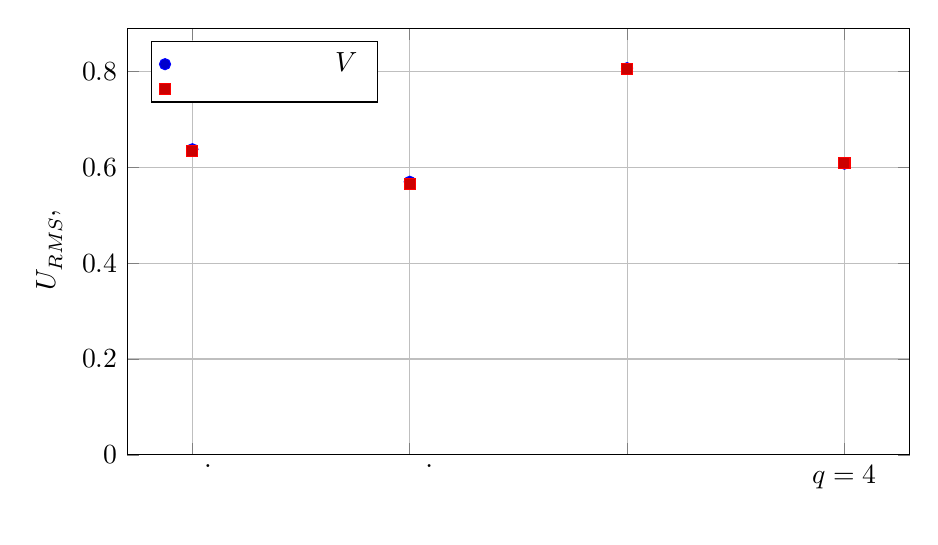
\begin{tikzpicture}
\begin{axis}[
width=0.95\textwidth,
height=7cm,
grid=both,
ymin=0,
ylabel={$U_{RMS}$, В},
xlabel={Номер формы сигнала},
xtick={1,2,3,4},
xticklabels={Гарм.,Треуг.,Меандр,$q=4$},
legend pos=north west
]
\addplot+[only marks, mark=*, error bars/.cd, y dir=both, y explicit]
coordinates {
(1,\UGarmTotal) +- (0,\ThetaACGarm)
(2,\UTriangularTotal) +- (0,\ThetaACTriangular)
(3,\UMeanderTotal) +- (0,\ThetaACMeander)
(4,\URectangularTotal) +- (0,\ThetaACRectangular)
};
\addlegendentry{Мультиметр с учетом $V_{\text{ср}}$}
\addplot+[only marks, mark=square*]
coordinates {
(1,\ProblemTwoGarmonicVRMSOne)
(2,\ProblemTwoTriangularVRMSOne)
(3,\ProblemTwoMeanderVRMSOne)
(4,\ProblemTwoRectangularVRMSOne)
};
\addlegendentry{Осциллограф}
\end{axis}
\end{tikzpicture}
\caption{Сравнение действующих значений напряжения по мультиметру и осциллографу}
\label{fig:rms-comparison}
\end{figure}

По рис.~\ref{fig:rms-comparison} видно, что порядок значений совпадает с ожидаемыми значениями для заданных форм сигналов. Наибольшее расхождение относится к гармоническому и треугольному сигналам, что связано с различием алгоритмов учета постоянной составляющей и вычисления действующего значения на приборах.

\fancyhead[L]{Задание $3$}
\section{Измерение методической погрешности из-за подключаемой нагрузки на выход генератора сигналов}

\subsection{Схема подключения и измерение сопротивления нагрузки}

Схема подключения низкоомной нагрузки представлена на рис.~\ref{fig:load-measure}.

\begin{figure}[H]
\centering
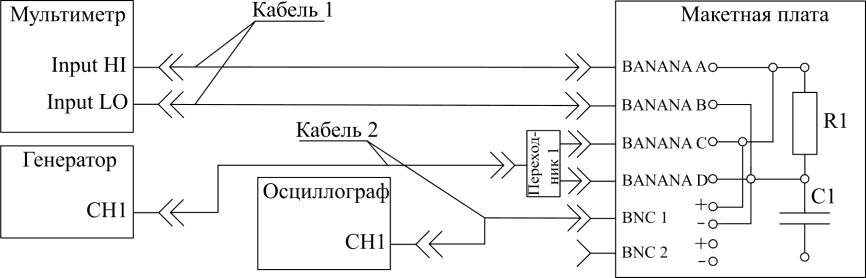
\includegraphics[width=0.92\textwidth]{02scheme.png}
\caption{Схема измерения напряжения генератора при подключенной низкоомной нагрузке}
\label{fig:load-measure}
\end{figure}

\begin{table}[H]
\caption{Протокол измерения сопротивления резистора RC-цепи}
\label{tab:a22}
\begin{tabularx}{\textwidth}{|C|C|C|C|}
\hline
\small Диапазон измерений, Ом & \small Скорость измерений, изм/с & \small Сила испытательного тока, мА & \small Показания мультиметра, Ом \\
\hline
$2000$ & $\S$ & $1$ & $\ProblemThreeResistance$ \\
\hline
\end{tabularx}
\end{table}

Погрешность измерения сопротивления
\begin{equation*}
\Theta_R=\pm1.1\sqrt{\theta_R^2+\theta_{2WR}^2}
\end{equation*}
\begin{equation*}
\Theta_R=\pm1.1\sqrt{\left(0.0002\cdot\ProblemThreeResistance+0.06\right)^2+0.2^2}
\end{equation*}
\begin{equation*}
\Theta_R\approx\pm\CalcFive{\ThetaR}\ \text{Ом}
\end{equation*}

\subsection{Измерение выходного сигнала при изменении нагрузки}

\begin{table}[H]
\caption{Протокол измерения выходного сигнала генератора при наличии низкоомной нагрузки}
\label{tab:a23}
\begin{tabularx}{\textwidth}{|p{4.5cm}|C|C|C|}
\hline
Генератор сигналов & $V_{pp}$: $\Vpp$ В & $V_{DC}$: $\VDC$ В & $f_\text{сигн}$: $\fpeval{\fSignal * 10^{-3}}$ кГц \\
\hline
Осциллограф & $K_{CH1}$: $\KCHone$ В/дел & $K_T$: $\KT$ мс/дел & \\
\hline
Мультиметр & Диапазон: $\Vrange$ В & $\nu$: $\S$ изм/с & $R_V$: \RVText \\
\hline
\small Форма сигнала --- гармонический & \multicolumn{2}{c|}{\raisebox{-0.5em}{Показания осциллографа}} & \small Показания мультиметра \\
\hline
Настройки нагрузки & $V_{pp1}$, В & $V_{RMS1}$, В & $V_{RMS2}$, В \\
\hline
Высокоомная нагрузка & $\ProblemThreeHighVppOne$ & $\ProblemThreeHighVRMSOne$ & $\ProblemThreeHighVRMSTwo$ \\
\hline
Нагрузка: $\fpeval{floor(\ProblemThreeResistance)}$ Ом & $\ProblemThreeLowVppOne$ & $\ProblemThreeLowVRMSOne$ & $\ProblemThreeLowVRMSTwo$ \\
\hline
\end{tabularx}
\end{table}

\subsection{Расчёт методической погрешности генератора}

Методическая погрешность генератора по \eqref{eq:gen-method}
\begin{equation*}
\gamma_{\text{мет}}=\frac{R_{\text{вых}}}{R_{\text{вых}}+R_{\text{н}}}\cdot100\%
\end{equation*}
\begin{equation*}
\gamma_{\text{мет}}=\frac{\RGenerator}{\RGenerator+\ProblemThreeResistance}\cdot100\%
\end{equation*}
\begin{equation}
\gamma_{\text{мет}}\approx\CalcTwo{\GeneratorDropRel*100}\%
\label{eq:gen-method-result}
\end{equation}

Ожидаемый размах на нагрузке без компенсации настройки выхода генератора по \eqref{eq:gen-load}
\begin{equation*}
V_{pp,\text{н}}=\ProblemThreeHighVppOne\cdot\frac{\ProblemThreeResistance}{\RGenerator+\ProblemThreeResistance}\approx\CalcFive{\GeneratorLoadVppCalc}\ \text{В}
\end{equation*}

Разность измеренных размахов при двух настройках нагрузки
\begin{equation*}
\Delta V_{pp}=|\ProblemThreeLowVppOne-\ProblemThreeHighVppOne|\approx\CalcFive{\GeneratorMeasuredDiffVpp}\ \text{В}
\end{equation*}

Относительная разность измеренных размахов
\begin{equation}
\delta_{\Delta V}=\frac{\GeneratorMeasuredDiffVpp}{\ProblemThreeHighVppOne}\cdot100\%\approx\CalcTwo{\GeneratorMeasuredDiffRel*100}\%
\label{eq:gen-diff-rel-result}
\end{equation}

\subsection{Вывод по влиянию нагрузочного сопротивления}

Настройка генератора на низкоомную нагрузку частично компенсирует влияние внутреннего сопротивления $R_{\text{вых}}=50$ Ом. Измеренная разность по \eqref{eq:gen-diff-rel-result} меньше расчетной оценки по \eqref{eq:gen-method-result}, что подтверждает работоспособность компенсации нагрузки генератора.

\fancyhead[L]{Задание $4$}
\section{Измерение частоты среза апериодического звена}

\subsection{Схемы измерения и параметры RC-цепи}

\begin{table}[H]
\caption{Протокол измерения ёмкости конденсатора RC-цепи}
\label{tab:a24}
\begin{tabularx}{\textwidth}{|C|C|C|}
\hline
\small Диапазон измерений, нФ & \small Сила испытательного тока, мА & \small Показания в режиме измерения ёмкости, нФ \\
\hline
$2$ & $1$ & $\fpeval{\ProblemFourCapacitance * 10^{9}}$ \\
\hline
\end{tabularx}
\end{table}

\begin{figure}[H]
\centering
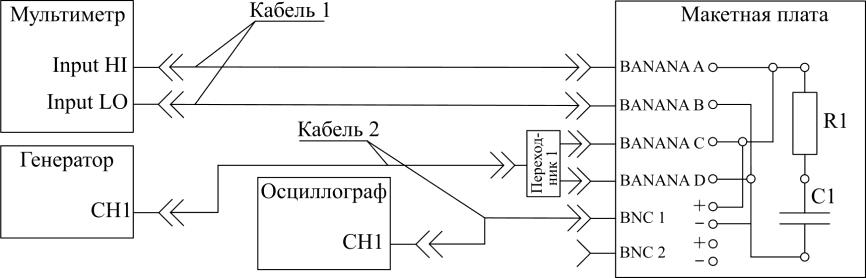
\includegraphics[width=0.92\textwidth]{03scheme.png}
\caption{Схема измерения напряжения генератора при наличии резистивной и емкостной нагрузок}
\label{fig:rc-load-measure}
\end{figure}

\begin{table}[H]
\caption{Протокол измерения выходного сигнала генератора при резистивной и ёмкостной нагрузках}
\label{tab:a25}
\begin{tabularx}{\textwidth}{|p{4.5cm}|C|C|C|}
\hline
Генератор сигналов & $V_{pp}$: $\Vpp$ В & $V_{DC}$: $\VDC$ В & $f_\text{сигн}$: $\fpeval{\fSignal * 10^{-3}}$ кГц \\
\hline
Осциллограф & $K_{CH1}$: $\KCHone$ В/дел & $K_T$: $\KT$ мс/дел & \\
\hline
Мультиметр & Диапазон: $\Vrange$ В & $\nu$: $\S$ изм/с & $R_V$: \RVText \\
\hline
\small Форма сигнала --- гармонический & \multicolumn{2}{c|}{\raisebox{-0.5em}{Показания осциллографа}} & \small Показания мультиметра \\
\hline
Настройки нагрузки & $V_{pp1}$, В & $V_{RMS1}$, В & $V_{RMS2}$, В \\
\hline
Нагрузка: $\fpeval{floor(\ProblemThreeResistance)}$ Ом & $\ProblemFourLowVppOne$ & $\ProblemFourLowVRMSOne$ & $\ProblemFourLowVRMSTwo$ \\
\hline
Высокоомная нагрузка & $\ProblemFourHighVppOne$ & $\ProblemFourHighVRMSOne$ & $\ProblemFourHighVRMSTwo$ \\
\hline
\end{tabularx}
\end{table}

\subsection{Расчётное и экспериментальное определение частоты среза}

Частота среза по \eqref{eq:fcut}
\begin{equation*}
f_{\text{ср}}=\frac{1}{2\pi RC}
\end{equation*}
\begin{equation*}
f_{\text{ср}}=\frac{1}{2\pi\cdot\ProblemThreeResistance\cdot\ProblemFourCapacitance}
\end{equation*}
\begin{equation*}
f_{\text{ср}}\approx\CalcThree{\FCutCalcKHz}\ \text{кГц}
\end{equation*}

Экспериментальная частота среза по \eqref{eq:sqrt2}
\begin{equation*}
\frac{V_{\text{вх}}}{V_{\text{вых}}}=\frac{\ProblemFourCutVinOne}{\ProblemFourCutVoutOne}\approx\CalcThree{\ProblemFourCutVinOne/\ProblemFourCutVoutOne}\approx\sqrt2
\end{equation*}

Экспериментальное значение частоты среза
\begin{equation*}
f_{\text{ср.изм}}\approx\CalcThree{\FCutExpKHz}\ \text{кГц}
\end{equation*}

\subsection{Протокол измерения частоты среза}

\begin{figure}[H]
\centering
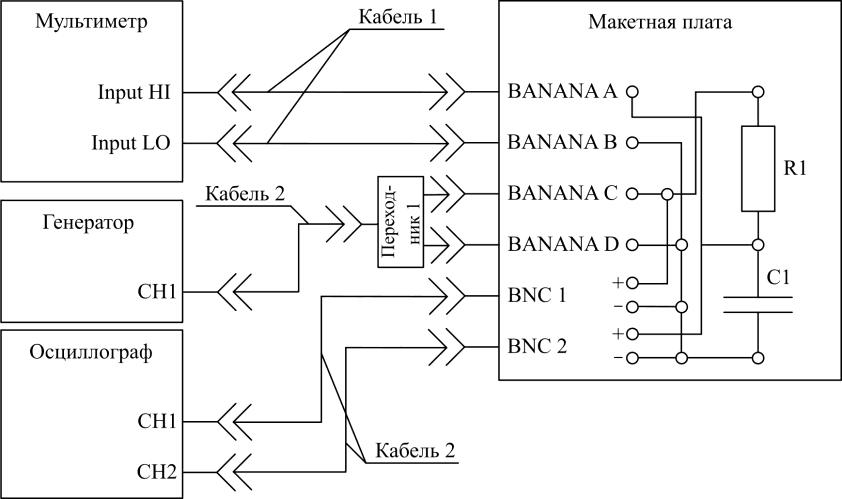
\includegraphics[width=0.92\textwidth]{04scheme.png}
\caption{Схема измерения частоты среза RC-цепи}
\label{fig:cutoff-measure}
\end{figure}

\begin{table}[H]
\caption{Протокол измерения частоты среза RC-цепи}
\label{tab:a26}
\begin{tabularx}{\textwidth}{|p{4.2cm}|C|C|C|}
\hline
Генератор сигналов & $V_{pp}$: $\Vpp$ В & $V_{DC}$: $\VDC$ В & $R_{\text{н}}$: HighZ \\
\hline
Мультиметр & Диапазон: $\Vrange$ В & $\nu$: $\S$ изм/с & $R_V$: \RVText \\
\hline
\small Форма сигнала --- гармонический & \multicolumn{2}{c|}{\raisebox{-0.5em}{Показания осциллографа, полный размах}} & \small Показания мультиметра \\
\hline
Частота, кГц & $V_{\text{вых}}$, В & $V_{\text{вх}}$, В & $V_{RMS2}$, В \\
\hline
$\CalcThree{\FTableSixOne}$ & $\ProblemFourCutVoutOne$ & $\ProblemFourCutVinOne$ & $\ProblemFourCutVRMSTwoOne$ \\
\hline
$\CalcThree{\FTableSixTwo}$ & $\ProblemFourCutVoutTwo$ & $\ProblemFourCutVinTwo$ & $\ProblemFourCutVRMSTwoTwo$ \\
\hline
$\CalcThree{\FTableSixThree}$ & $\ProblemFourCutVoutThree$ & $\ProblemFourCutVinThree$ & $\ProblemFourCutVRMSTwoThree$ \\
\hline
$\CalcThree{\FTableSixFour}$ & $\ProblemFourCutVoutFour$ & $\ProblemFourCutVinFour$ & $\ProblemFourCutVRMSTwoFour$ \\
\hline
$\CalcThree{\FTableSixFive}$ & $\ProblemFourCutVoutFive$ & $\ProblemFourCutVinFive$ & $\ProblemFourCutVRMSTwoFive$ \\
\hline
$\CalcThree{\FTableSixSix}$ & $\ProblemFourCutVoutSix$ & $\ProblemFourCutVinSix$ & $\ProblemFourCutVRMSTwoSix$ \\
\hline
$\CalcThree{\FTableSixSeven}$ & $\ProblemFourCutVoutSeven$ & $\ProblemFourCutVinSeven$ & $\ProblemFourCutVRMSTwoSeven$ \\
\hline
$\CalcThree{\FTableSixEight}$ & $\ProblemFourCutVoutEight$ & $\ProblemFourCutVinEight$ & $\ProblemFourCutVRMSTwoEight$ \\
\hline
$\CalcThree{\FTableSixNine}$ & $\ProblemFourCutVoutNine$ & $\ProblemFourCutVinNine$ & $\ProblemFourCutVRMSTwoNine$ \\
\hline
$\CalcThree{\FTableSixTen}$ & $\ProblemFourCutVoutTen$ & $\ProblemFourCutVinTen$ & $\ProblemFourCutVRMSTwoTen$ \\
\hline
$\CalcThree{\FTableSixEleven}$ & $\ProblemFourCutVoutEleven$ & $\ProblemFourCutVinEleven$ & $\ProblemFourCutVRMSTwoEleven$ \\
\hline
\end{tabularx}
\end{table}

\subsection{Логарифмический график АЧХ}

\begin{figure}[H]
\centering
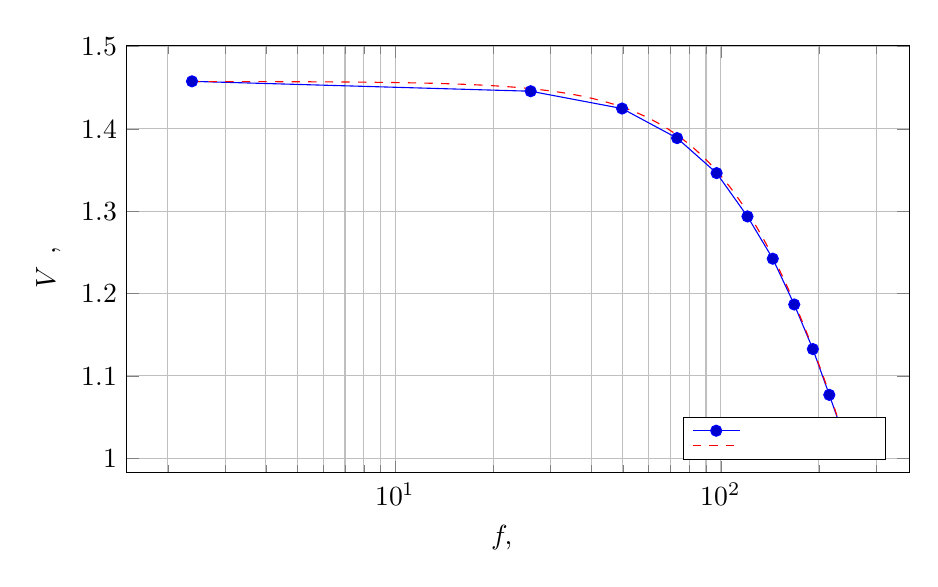
\begin{tikzpicture}
\begin{axis}[
width=0.95\textwidth,
height=7cm,
xmode=log,
grid=both,
xlabel={$f$, кГц},
ylabel={$V_{\text{вых}}$, В},
legend pos=south east
]
\addplot+[mark=*] coordinates {
(\FTableSixOne,\ProblemFourCutVoutOne)
(\FTableSixTwo,\ProblemFourCutVoutTwo)
(\FTableSixThree,\ProblemFourCutVoutThree)
(\FTableSixFour,\ProblemFourCutVoutFour)
(\FTableSixFive,\ProblemFourCutVoutFive)
(\FTableSixSix,\ProblemFourCutVoutSix)
(\FTableSixSeven,\ProblemFourCutVoutSeven)
(\FTableSixEight,\ProblemFourCutVoutEight)
(\FTableSixNine,\ProblemFourCutVoutNine)
(\FTableSixTen,\ProblemFourCutVoutTen)
(\FTableSixEleven,\ProblemFourCutVoutEleven)
};
\addlegendentry{Измеренные точки}
\addplot+[domain=\FLowKHz:\FCutExpKHz, samples=200, no marks, dashed] {\ProblemFourCutVinEleven/(sqrt(1+(x/\FCutCalcKHz)^2))};
\addlegendentry{Модель ФНЧ}
\end{axis}
\end{tikzpicture}
\caption{Логарифмический график определения частоты среза RC-цепи}
\label{fig:ach-cutoff}
\end{figure}

\subsection{Оценка погрешности частоты среза}

Относительное расхождение расчетной и экспериментальной частоты
\begin{equation*}
\delta_f=\frac{|f_{\text{ср.изм}}-f_{\text{ср}}|}{f_{\text{ср}}}\cdot100\%
\end{equation*}
\begin{equation}
\delta_f=\frac{|\FCutExp-\FCutCalc|}{\FCutCalc}\cdot100\%\approx\CalcTwo{abs(\FCutExp-\FCutCalc)/\FCutCalc*100}\%
\label{eq:fcut-diff}
\end{equation}

Погрешность косвенного определения частоты среза по \eqref{eq:fcut-error}
\begin{equation}
\frac{\Theta_f}{f_{\text{ср}}}=\sqrt{\left(\frac{\ThetaR}{\ProblemThreeResistance}\right)^2+\left(0.0136\right)^2}\approx\CalcTwo{\ThetaFRel*100}\%
\label{eq:fcut-error-result-rel}
\end{equation}
\begin{equation*}
\Theta_f\approx\CalcThree{\ThetaFKHz}\ \text{кГц}
\end{equation*}

Расхождение по \eqref{eq:fcut-diff} меньше оценки косвенной погрешности по \eqref{eq:fcut-error-result-rel}, поэтому расчетное и экспериментальное значения частоты среза согласуются.

\fancyhead[L]{Задание $5$}
\section{Измерение напряжения переменного тока на выходе ФНЧ}

\subsection{Схема ФНЧ и характерные частоты}

Схема ФНЧ представлена на рис.~\ref{fig:lpf-scheme}. Выходное напряжение снимается с конденсатора.

\begin{figure}[H]
\centering
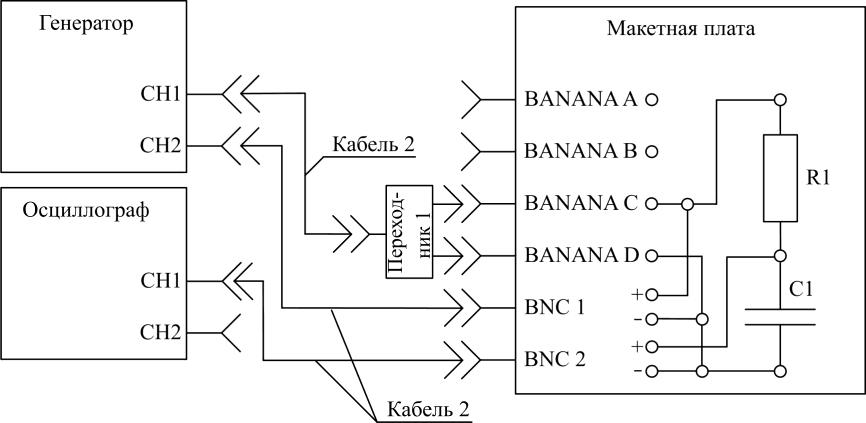
\includegraphics[width=0.92\textwidth]{05scheme.png}
\caption{Схема RC-цепи в режиме фильтра низких частот}
\label{fig:lpf-scheme}
\end{figure}

Низкая частота
\begin{equation*}
f_{0.01}=0.01f_{\text{ср}}=0.01\cdot\FCutCalcKHz\approx\CalcThree{\FLowKHz}\ \text{кГц}
\end{equation*}

Высокая частота
\begin{equation*}
f_{100}=100f_{\text{ср}}=100\cdot\FCutCalcKHz\approx\CalcTwo{\FHighKHz}\ \text{кГц}=\CalcThree{\FHighMHz}\ \text{МГц}
\end{equation*}

\subsection{Протокол измерения выходного напряжения ФНЧ}

\begin{table}[H]
	\caption{Протокол измерения напряжения переменного тока на выходе ФНЧ}
	\begin{tabularx}{\textwidth}{|p{3.5cm}|C|C|C|C|}
		\hline
		\multirow{3}{=}{Генератор сигналов:} & $V_{CH1}$: $\Vpp$ В & $V_{CH2}$: $\Vpp$ В & \multicolumn{2}{p{6cm}|}{\multirow{2}{=}{\centering Показания осциллографа}} \\
		\cline{2-3}
		& $V_{DC1}$: $\VDC$ В & $V_{DC2}$: $\VDC$ В & \multicolumn{2}{p{6cm}|}{ } \\
		\cline{2-5}
		& $f_{CH1}$, кГц & $f_{CH2}$, кГц & $V_{\text{вых}}$, В & $V_{\text{вх}}$, В \\
		\hline
		\multirow{3}{=}{Форма сигнала — гармонический} &
		$0.01f_{\text{ср}}$: $\CalcThree{\FLowKHz}$ &
		$0.01f_{\text{ср}}$: $\CalcThree{\FLowKHz}$ &
		$\ProblemFiveLPFVoutOne$ & $\ProblemFiveLPFVinOne$ \\
		\cline{2-5}
		&
		$0.01f_{\text{ср}}$: $\CalcThree{\FLowKHz}$ &
		$f_{\text{ср}}$: $\CalcThree{\FCutExpKHz}$ &
		$\ProblemFiveLPFVoutTwo$ & $\ProblemFiveLPFVinTwo$ \\
		\cline{2-5}
		&
		$0.01f_{\text{ср}}$: $\CalcThree{\FLowKHz}$ &
		$100f_{\text{ср}}$: $\CalcTwo{\FHighKHz}$ &
		$\ProblemFiveLPFVoutThree$ & $\ProblemFiveLPFVinThree$ \\
		\hline
	\end{tabularx}
\end{table}

\subsection{Оценка ослабления составляющих сигнала}

Коэффициенты передачи ФНЧ в характерных точках
\begin{equation*}
K_{\text{ФНЧ}}(0.01f_{\text{ср}})=\frac{1}{\sqrt{1+0.01^2}}\approx\CalcFour{1/sqrt(1+0.01^2)}
\end{equation*}
\begin{equation*}
K_{\text{ФНЧ}}(f_{\text{ср}})=\frac{1}{\sqrt2}\approx\CalcFour{1/sqrt(2)}
\end{equation*}
\begin{equation*}
K_{\text{ФНЧ}}(100f_{\text{ср}})=\frac{1}{\sqrt{1+100^2}}\approx\CalcFour{1/sqrt(1+100^2)}
\end{equation*}

Измеренные отношения размахов
\begin{equation*}
\frac{V_{\text{вых}}}{V_{\text{вх}}}=\frac{\ProblemFiveLPFVoutOne}{\ProblemFiveLPFVinOne}\approx\CalcThree{\ProblemFiveLPFVoutOne/\ProblemFiveLPFVinOne}
\end{equation*}
\begin{equation*}
\frac{V_{\text{вых}}}{V_{\text{вх}}}=\frac{\ProblemFiveLPFVoutTwo}{\ProblemFiveLPFVinTwo}\approx\CalcThree{\ProblemFiveLPFVoutTwo/\ProblemFiveLPFVinTwo}
\end{equation*}
\begin{equation*}
\frac{V_{\text{вых}}}{V_{\text{вх}}}=\frac{\ProblemFiveLPFVoutThree}{\ProblemFiveLPFVinThree}\approx\CalcThree{\ProblemFiveLPFVoutThree/\ProblemFiveLPFVinThree}
\end{equation*}

\subsection{Анализ формы выходного сигнала}

\begin{figure}[H]
\centering
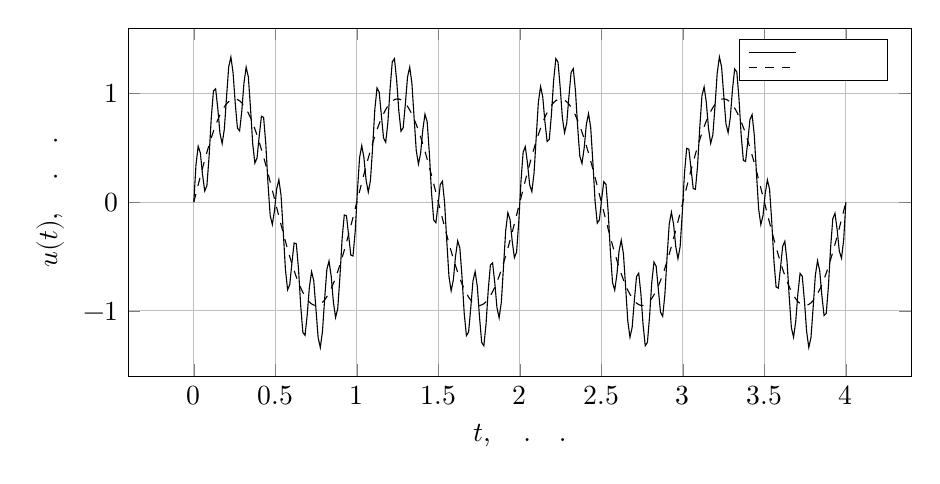
\begin{tikzpicture}
\begin{axis}[
width=0.95\textwidth,
height=6cm,
grid=both,
xlabel={$t$, усл. ед.},
ylabel={$u(t)$, усл. ед.},
legend pos=north east,
ymin=-1.6,ymax=1.6
]
\addplot[domain=0:4, samples=300] {sin(deg(2*pi*x))+0.35*sin(deg(20*pi*x))};
\addplot[domain=0:4, samples=300, dashed] {0.95*sin(deg(2*pi*x))};
\legend{Вход,Выход ФНЧ}
\end{axis}
\end{tikzpicture}
\caption{Схематическое изображение входного и выходного сигналов ФНЧ}
\label{fig:lpf-wave}
\end{figure}

ФНЧ сохраняет низкочастотную составляющую и подавляет высокочастотную составляющую. При подаче суммы двух сигналов полный размах выходного напряжения уменьшается примерно до половины исходного размаха, но не обращается в ноль.

\fancyhead[L]{Задание $6$}
\section{Измерение напряжения переменного тока на выходе ФВЧ}

\subsection{Схема ФВЧ и протокол измерения}

Схема ФВЧ представлена на рис.~\ref{fig:hpf-scheme}. Выходное напряжение снимается с резистора.

\begin{figure}[H]
\centering
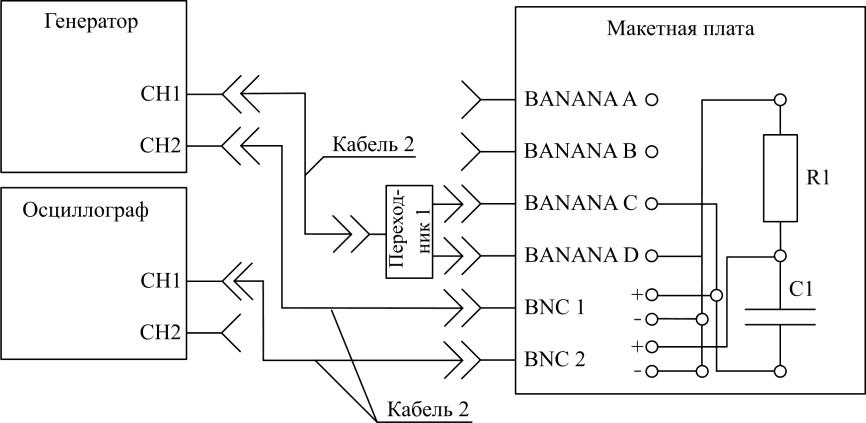
\includegraphics[width=0.92\textwidth]{06scheme.png}
\caption{Схема RC-цепи в режиме фильтра высоких частот}
\label{fig:hpf-scheme}
\end{figure}

\begin{table}[H]
	\caption{Протокол измерения напряжения переменного тока на выходе ФВЧ}
	\begin{tabularx}{\textwidth}{|p{3.5cm}|C|C|C|C|}
		\hline
		\multirow{3}{=}{Генератор сигналов:} & $V_{CH1}$: $\Vpp$ В & $V_{CH2}$: $\Vpp$ В & \multicolumn{2}{p{6cm}|}{\multirow{2}{=}{\centering Показания осциллографа}} \\
		\cline{2-3}
		& $V_{DC1}$: $\VDC$ В & $V_{DC2}$: $\VDC$ В & \multicolumn{2}{p{6cm}|}{ } \\
		\cline{2-5}
		& $f_{CH1}$, кГц & $f_{CH2}$, кГц & $V_{\text{вых}}$, В & $V_{\text{вх}}$, В \\
		\hline
		\multirow{3}{=}{Форма сигнала — гармонический} &
		$100f_{\text{ср}}$: $\CalcTwo{\FHighKHz}$ &
		$100f_{\text{ср}}$: $\CalcTwo{\FHighKHz}$ &
		$\ProblemSixHPFVoutOne$ & $\ProblemSixHPFVinOne$ \\
		\cline{2-5}
		&
		$100f_{\text{ср}}$: $\CalcTwo{\FHighKHz}$ &
		$f_{\text{ср}}$: $\CalcThree{\FCutExpKHz}$ &
		$\ProblemSixHPFVoutTwo$ & $\ProblemSixHPFVinTwo$ \\
		\cline{2-5}
		&
		$100f_{\text{ср}}$: $\CalcTwo{\FHighKHz}$ &
		$0.01f_{\text{ср}}$: $\CalcThree{\FLowKHz}$ &
		$\ProblemSixHPFVoutThree$ & $\ProblemSixHPFVinThree$ \\
		\hline
	\end{tabularx}
\end{table}

\subsection{Оценка ослабления составляющих сигнала}

Коэффициенты передачи ФВЧ в характерных точках
\begin{equation*}
K_{\text{ФВЧ}}(100f_{\text{ср}})=\frac{100}{\sqrt{1+100^2}}\approx\CalcFour{100/sqrt(1+100^2)}
\end{equation*}
\begin{equation*}
K_{\text{ФВЧ}}(f_{\text{ср}})=\frac{1}{\sqrt2}\approx\CalcFour{1/sqrt(2)}
\end{equation*}
\begin{equation*}
K_{\text{ФВЧ}}(0.01f_{\text{ср}})=\frac{0.01}{\sqrt{1+0.01^2}}\approx\CalcFour{0.01/sqrt(1+0.01^2)}
\end{equation*}

Измеренные отношения размахов
\begin{equation*}
\frac{V_{\text{вых}}}{V_{\text{вх}}}=\frac{\ProblemSixHPFVoutOne}{\ProblemSixHPFVinOne}\approx\CalcThree{\ProblemSixHPFVoutOne/\ProblemSixHPFVinOne}
\end{equation*}
\begin{equation*}
\frac{V_{\text{вых}}}{V_{\text{вх}}}=\frac{\ProblemSixHPFVoutTwo}{\ProblemSixHPFVinTwo}\approx\CalcThree{\ProblemSixHPFVoutTwo/\ProblemSixHPFVinTwo}
\end{equation*}
\begin{equation*}
\frac{V_{\text{вых}}}{V_{\text{вх}}}=\frac{\ProblemSixHPFVoutThree}{\ProblemSixHPFVinThree}\approx\CalcThree{\ProblemSixHPFVoutThree/\ProblemSixHPFVinThree}
\end{equation*}

\subsection{Анализ формы выходного сигнала}

\begin{figure}[H]
\centering
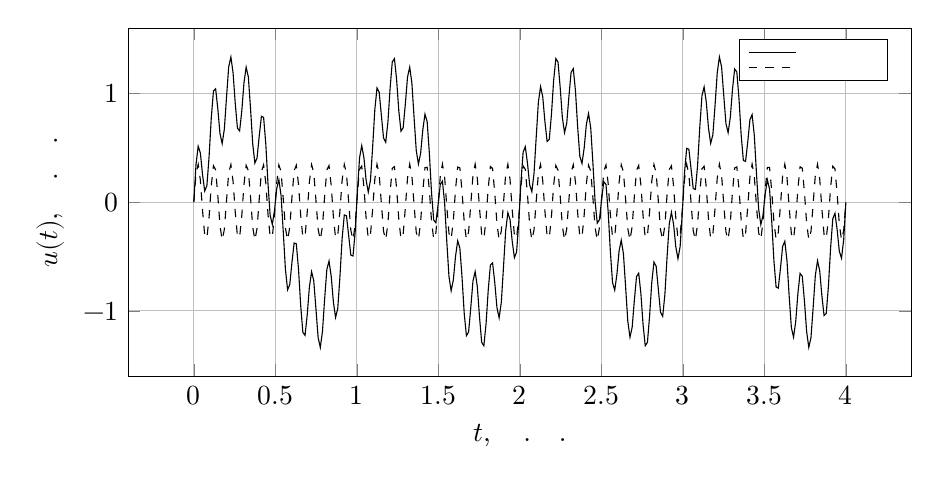
\begin{tikzpicture}
\begin{axis}[
width=0.95\textwidth,
height=6cm,
grid=both,
xlabel={$t$, усл. ед.},
ylabel={$u(t)$, усл. ед.},
legend pos=north east,
ymin=-1.6,ymax=1.6
]
\addplot[domain=0:4, samples=300] {sin(deg(2*pi*x))+0.35*sin(deg(20*pi*x))};
\addplot[domain=0:4, samples=300, dashed] {0.35*sin(deg(20*pi*x))};
\legend{Вход,Выход ФВЧ}
\end{axis}
\end{tikzpicture}
\caption{Схематическое изображение входного и выходного сигналов ФВЧ}
\label{fig:hpf-wave}
\end{figure}

ФВЧ сохраняет высокочастотную составляющую и подавляет низкочастотную составляющую. При подаче суммы двух сигналов полный размах выходного напряжения уменьшается примерно до половины исходного размаха, потому что на выходе остается высокочастотная часть сигнала.

\section*{Выводы}
\addcontentsline{toc}{section}{Выводы}
\fancyhead[L]{Выводы}

В ходе лабораторной работы были выполнены измерения параметров сигналов с использованием генератора Rigol DG$1022$Z, мультиметра Rigol DM$3058$ и осциллографа Rigol MSO$5102$.

Сигналы стандартной формы при настройках $V_{pp}=\Vpp$ В, $V_{DC}=\VDC$ В и $f=\fpeval{\fSignal*10^{-3}}$ кГц имели значения полного размаха и действующего напряжения, приведенные в табл.~\ref{tab:a21}. Учет постоянной составляющей по \eqref{eq:utotal} позволил согласовать показания мультиметра с физическим смыслом полного действующего значения.

Сопротивление резистора RC-цепи
\begin{equation*}
R=(\ProblemThreeResistance\pm\CalcFive{\ThetaR})\ \text{Ом}
\end{equation*}

Методическая погрешность генератора при подключении нагрузки $R=\ProblemThreeResistance$ Ом
\begin{equation*}
\gamma_{\text{мет}}\approx\CalcTwo{\GeneratorDropRel*100}\%
\end{equation*}

Емкость конденсатора RC-цепи
\begin{equation*}
C=\fpeval{\ProblemFourCapacitance*10^9}\ \text{нФ}
\end{equation*}

Расчетная частота среза RC-цепи
\begin{equation*}
f_{\text{ср}}\approx\CalcThree{\FCutCalcKHz}\ \text{кГц}
\end{equation*}

Экспериментальная частота среза
\begin{equation*}
f_{\text{ср.изм}}\approx\CalcThree{\FCutExpKHz}\ \text{кГц}
\end{equation*}

Расхождение расчетного и экспериментального значений равно 
$\CalcTwo{abs(\FCutExp-\FCutCalc)/\FCutCalc*100}\%$, что меньше оценки косвенной 
погрешности $\CalcTwo{\ThetaFRel*100}\%$. Частота среза определена корректно.

При исследовании ФНЧ низкочастотная составляющая $0{,}01f_{\text{ср}}$ проходила
 почти без ослабления, составляющая на частоте среза ослаблялась примерно до уровня 
 $1/\sqrt2$, а высокочастотная составляющая $100f_{\text{ср}}$ подавлялась. 
 При исследовании ФВЧ наблюдалась обратная картина.


\pagebreak
\section*{Список использованной литературы}
\addcontentsline{toc}{section}{Список использованной литературы}
\fancyhead[L]{Список использованной литературы}

\begin{enumerate}
\item Калеев Д. В. Метрология и электрорадиоизмерения : лабораторный практикум. --- М. : МИЭТ, 2025. --- 184 с. : ил.
\item User's Guide RIGOL DM3058/DM3058E Digital Multimeter. --- RIGOL Technologies.
\item Data Sheet RIGOL DG1000Z Series Function/Arbitrary Waveform Generator. --- RIGOL Technologies.
\item Описание типа средства измерений. Осциллографы цифровые серии MSO5000. --- RIGOL Technologies.
\end{enumerate}

\pagebreak
\section*{Приложение А}
\addcontentsline{toc}{section}{Приложение А}
\fancyhead[L]{Приложение А}

\end{document}
